\documentclass[14pt,a4paper]{extarticle}

% Шрифты и русский язык
\usepackage{fontspec}
\setmainfont{Times New Roman}
\setmonofont{JetBrains Mono}
\usepackage[russian]{babel}
\usepackage{titlesec}

% Заголовки разделов
\titleformat{\section}
  {\normalfont\fontsize{14pt}{17pt}\selectfont\bfseries}
  {\thesection}{1em}{}

% Заголовки подразделов
\titleformat{\subsection}
  {\normalfont\fontsize{13pt}{16pt}\selectfont\bfseries}
  {\thesubsection}{1em}{}

% Отступы до и после заголовков
\titlespacing*{\section}{0pt}{12pt}{6pt}
\titlespacing*{\subsection}{0pt}{10pt}{5pt}

% Поля страницы
\usepackage[left=25mm,right=20mm,top=20mm,bottom=20mm]{geometry}

% Таблицы, изображения и ссылки
\usepackage{longtable,array,graphicx,hyperref}
\hypersetup{hidelinks}

% Абзацы и таблицы
\setlength{\parindent}{0pt}
\setlength{\parskip}{6pt}
\renewcommand{\arraystretch}{1.12}

% Подсветка синтаксиса
\usepackage{xcolor}
\usepackage{listings}

% Цвета светлой темы CLion
\definecolor{codeBlue}{HTML}{0033B3}
\definecolor{codeGreen}{HTML}{067D17}
\definecolor{codeGray}{HTML}{808080}
\definecolor{codeText}{HTML}{202124}
\definecolor{codeBorder}{HTML}{E0E0E0}

% Стиль листинга
\lstdefinestyle{clion}{
    backgroundcolor=\color{white},
    basicstyle=\ttfamily\fontsize{10.5pt}{13pt}\selectfont\color{codeText},
    keywordstyle=\color{codeBlue},
    stringstyle=\color{codeGreen},
    commentstyle=\color{codeGray}\itshape,
    identifierstyle=\color{codeText},
    rulecolor=\color{codeBorder},
    breaklines=true,
    breakatwhitespace=false,
    keepspaces=true,
    showstringspaces=false,
    columns=fullflexible,
    tabsize=4
}

\lstset{style=clion}
\usepackage{amsmath}
\usepackage{float}
\usepackage{caption}
\captionsetup{font=small}

\newcommand{\code}[1]{{\ttfamily\fontsize{10.5pt}{13pt}\selectfont #1}}
\setlength{\emergencystretch}{1em}
\begin{document}
\begin{center}
\textbf{Лабораторная работа №4}\\[4pt]
Построение сеточной модели звёзд окрестности Солнца
\end{center}

\section{Задание}
Ограничить сеточные модели рамками модели, куба с ребром 1000 св.лет.

Уточнение: Диаграмма Вороного должна быть обрезана по граням даммикуба рамок модели. Для визуализации 6-ти сечений мозаики полиэдральной сетки.

\section{Подготовка звёздного каталога}
Использован каталог HYG v2 (\code{hygxyz.csv}, David Nash / Astronexus), содержащий 119\,617 записей. Отбор по расстоянию выполнен с коэффициентом перевода из парсеков в световые годы $k=3{,}262$:
\begin{lstlisting}[language=SQL]
SELECT StarID, Distance*3.262 AS Light_Years,
       Spectrum, X, Y, Z
FROM hyg
WHERE Distance*3.262 <= 500;
\end{lstlisting}
Получено 42\,748 записей. Результат сохранён в \code{500ly.sqlite}. Для семи классов выполняется запрос вида:
\begin{lstlisting}[language=SQL]
SELECT StarID, X, Y, Z FROM hyg
WHERE Spectrum LIKE 'O%';
\end{lstlisting}
Оператор \code{LIKE} в SQLite учитывает начальные латинские буквы без различия регистра. Получены 40\,592 записи классов O, B, A, F, G, K, M; 2\,156 записей с другими или отсутствующими начальными обозначениями не включены в эти семь сеток. Спектральные обозначения трактуются по указанному правилу фильтрации; физическая переклассификация звёзд не выполняется.

Координаты каталога, как и расстояния, заданы в парсеках. Для геометрических расчётов преобразованы все три координаты:
\[
 (x,y,z)_{\text{св. лет}}=3{,}262\,(X,Y,Z)_{\text{пк}}.
\]
Начало координат совпадает с Солнцем. Ось $X$ направлена к точке весеннего равноденствия, ось $Z$ --- к северному полюсу мира, ось $Y$ --- в направлении прямого восхождения $6$ ч. Область модели:
\[
 C=\{(x,y,z): -500\leq x,y,z\leq500\}\quad\text{(св. лет)}.
\]
Отбор звёзд производится по шару радиуса 500 св. лет, а ограничение ячеек --- по кубу. Поэтому углы куба содержат продолжения ячеек ближайших звёзд, хотя самих отобранных звёзд там нет.

Совпадающие координаты объединены перед тетраэдрализацией. Все исходные записи сохранены, а таблица \code{catalogue} связывает \code{StarID} с индексом геометрического узла \code{NodeID}. Объединено 14 повторных положений: одно в F, одно в G, два в K и десять в M.

\begin{table}[ht]
\centering\small
\caption{Состав входных данных и тетраэдрализации}
\begin{tabular}{c|r|r|r|r}
Класс & Записей & Узлов & Тетраэдров & Рёбер Делоне\\\hline
O & 7 & 7 & 7 & 18 \\
B & 702 & 702 & 4207 & 5004 \\
A & 4845 & 4845 & 31574 & 36674 \\
F & 14292 & 14291 & 95000 & 109638 \\
G & 11942 & 11941 & 79351 & 91536 \\
K & 6720 & 6718 & 44275 & 51234 \\
M & 2084 & 2074 & 13554 & 15682

\end{tabular}
\end{table}

\section{Расчёт и ограничение сеток}
\subsection{Вызов TetGen}
Для каждого класса создан ASCII-файл \code{.node}. Его первая строка содержит число узлов, размерность 3, число атрибутов 0 и число маркеров 0. Индексы геометрических узлов непрерывны и начинаются с нуля; идентификаторы каталога хранятся отдельно.

Расчёт выполнен библиотекой \code{\_tetgenDLL.dll} из приложенного архива. Консольная оболочка \code{tetgen\_cli.exe} считывает узлы, вызывает \code{tetrahedralize} с ключами \code{zvfenQ} и сохраняет массивы результата. Ключ \code{z} задаёт нумерацию с нуля, \code{v} --- диаграмму Вороного, \code{f} --- все треугольные грани, \code{e} --- рёбра, \code{n} --- соседство тетраэдров, \code{Q} --- краткий вывод.

В девяти файлах каждого класса сохранены вершины, рёбра, грани, тетраэдры и соседство Делоне, а также вершины, рёбра, грани и ячейки Вороного. Для класса O получены 7 тетраэдров, 18 рёбер Делоне, 7 вершин и 19 рёбер Вороного, включая 10 неограниченных лучей. Эти результаты соответствуют геометрии семи исходных звёзд класса O.

Все вершины Делоне лежат внутри куба, а куб выпуклый. Следовательно, каждый тетраэдр и каждое его ребро также целиком лежат в кубе. Добавлять фиктивные звёзды в углах куба не требуется: это изменило бы исходную диаграмму Вороного.

\subsection{Отсечение отрезков и лучей}
Ребро Вороного записывается параметрически:
\[
 q(t)=a+td,
 \qquad t\in[0,1]\ \text{для отрезка},\qquad
 t\in[0,+\infty)\ \text{для луча}.
\]
Для каждой координаты пересекается допустимый интервал параметра с условием $-500\leq a_j+td_j\leq500$. При $d_j\neq0$ его границы равны:
\[
 t_j^- =\min\left(\frac{-500-a_j}{d_j},\frac{500-a_j}{d_j}\right),\quad
 t_j^+ =\max\left(\frac{-500-a_j}{d_j},\frac{500-a_j}{d_j}\right).
\]
При $d_j=0$ ребро отбрасывается только тогда, когда $a_j$ находится вне соответствующего слоя куба. Пустое пересечение интервалов означает отсутствие видимой части. Такой алгоритм сохраняет и отрезок, пересекающий куб при обеих внешних конечных точках. Для O куб пересекают 6 из 10 лучей.

При экспорте результатов приложенной DLL нормали граничных лучей развёрнуты в наружное направление. Ориентация проверена по условию трёх равноудалённых ближайших звёзд на каждом луче.

Одного отсечения исходных рёбер недостаточно для получения мозаики на гранях: необходимо построить новые границы ячеек в плоскостях куба.

\subsection{Замыкание ячеек на гранях куба}
Для звезды $p_i$ ограниченная ячейка определяется пересечением полупространств:
\[
 V_i^C=C\cap\bigcap_{j\neq i}
 \left\{x:\;2(p_j-p_i)\cdot x\leq
       \|p_j\|^2-\|p_i\|^2\right\}.
\]
В расчёте используются соседи $p_i$ по рёбрам Делоне: остальные ограничения избыточны. В локальных координатах $y=x-p_i$ неравенство принимает устойчивую к смещению форму
\[
 \frac{p_j-p_i}{\|p_j-p_i\|}\cdot y
 \leq\frac{\|p_j-p_i\|}{2}.
\]
К этим условиям добавлены шесть плоскостей куба. Вершины пересечения вычислены методом \code{HalfspaceIntersection}; точка $y=0$ служит внутренней опорной точкой. Из вершин на каждой плоскости $x_j=\pm500$ построен выпуклый многоугольник. Его рёбра добавлены к отсечённым исходным рёбрам Вороного. Общие рёбра граничных многоугольников объединены с округлением координат до $10^{-6}$ св. года только для ключа сопоставления; сохраняемые координаты остаются вещественными.

На каждой грани получена мозаика пересечений трёхмерных ячеек, а не двумерная диаграмма проекций звёзд. Во втором случае потерялась бы составляющая расстояния, перпендикулярная грани, и результат был бы другим.

\begin{figure}[p]
\centering
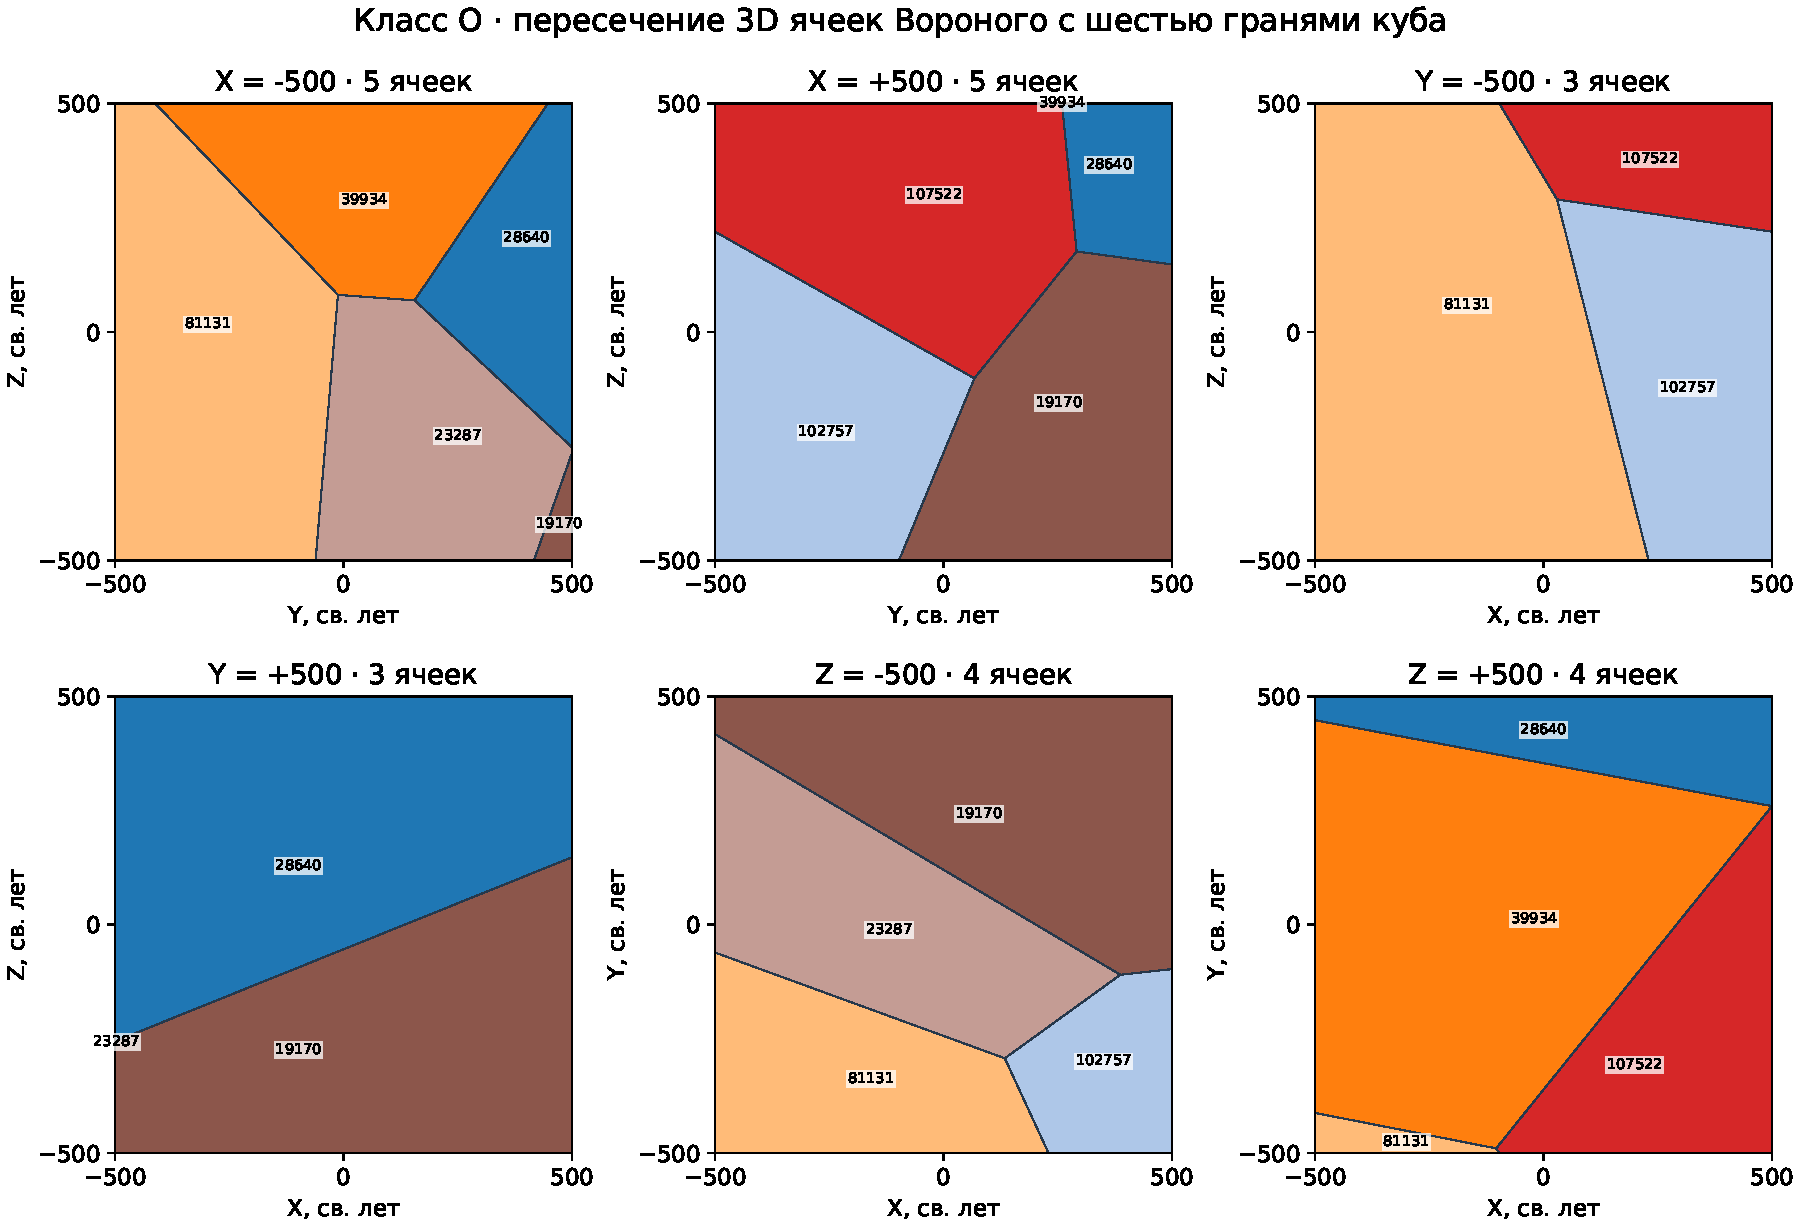
\includegraphics[width=\linewidth]{images/sections-O-plot.pdf}
\caption{Шесть точных сечений для класса O. Внутри многоугольников указаны StarID. Каждый квадрат имеет сторону 1000 св. лет.}
\end{figure}

\begin{table}[ht]
\centering\small
\caption{Граничные многоугольники ячеек Вороного}
\begin{tabular}{c|rrrrrr|r}
Класс & $X-$ & $X+$ & $Y-$ & $Y+$ & $Z-$ & $Z+$ & Всего\\\hline
O & 5 & 5 & 3 & 3 & 4 & 4 & 24 \\
B & 35 & 27 & 50 & 51 & 52 & 40 & 255 \\
A & 104 & 104 & 135 & 161 & 124 & 129 & 757 \\
F & 166 & 152 & 147 & 154 & 193 & 152 & 964 \\
G & 125 & 123 & 116 & 101 & 122 & 119 & 706 \\
K & 113 & 116 & 108 & 106 & 109 & 106 & 658 \\
M & 22 & 26 & 25 & 21 & 23 & 23 & 140

\end{tabular}
\end{table}

\clearpage
\section{Приложение визуализации}
Разработано приложение C++Builder / VCL / GLScene. Кнопка Start проверяет наличие 14 баз SQLite и загружает геометрию каждого класса в оперативную память. После загрузки доступны три режима: звёзды-точки, рёбра тетраэдрализации Делоне и ограниченная кубом диаграмма Вороного. Переключатели классов позволяют одновременно выводить несколько сеток; каждая построена отдельно по своему спектральному классу.

Компонент \code{TGLPoints} отображает звёзды, \code{TGLLines} --- независимые отрезки рёбер, \code{TGLSceneViewer} --- сцену. Мышью изменяется ракурс, колесом --- масштаб. В правой панели показаны фактические числа отображаемых звёзд и рёбер. Каркас куба задаёт границы модели в световых годах.

Кнопка «Шесть сечений на гранях» открывает форму с шестью мозаиками и выбором класса. Мозаики заранее рассчитаны по тем же граничным многоугольникам, которые сохранены в SQLite. Цвет в этой форме различает ячейки; в основной трёхмерной сцене цвет обозначает спектральный класс.

Форма Data предоставляет выбор любой из 14 баз и таблицы внутри неё. Отображение постраничное, по 500 записей, с указанием полного числа строк. Базы открываются только для чтения. В базах Делоне находятся таблицы \code{node}, \code{edge}, \code{face}, \code{ele}, \code{neigh}, \code{catalogue}; в базах Вороного --- \code{node}, \code{edge}, \code{face}, \code{cell}, а также \code{clipped\_edges}, \code{caps}, \code{cell\_volume}. Для граней и ячеек переменной длины список индексов сохранён в текстовом поле \code{members}. Таблица \code{caps} содержит номер грани куба, узел, StarID, площадь и упорядоченные вершины многоугольника.

\begin{figure}[ht]
\centering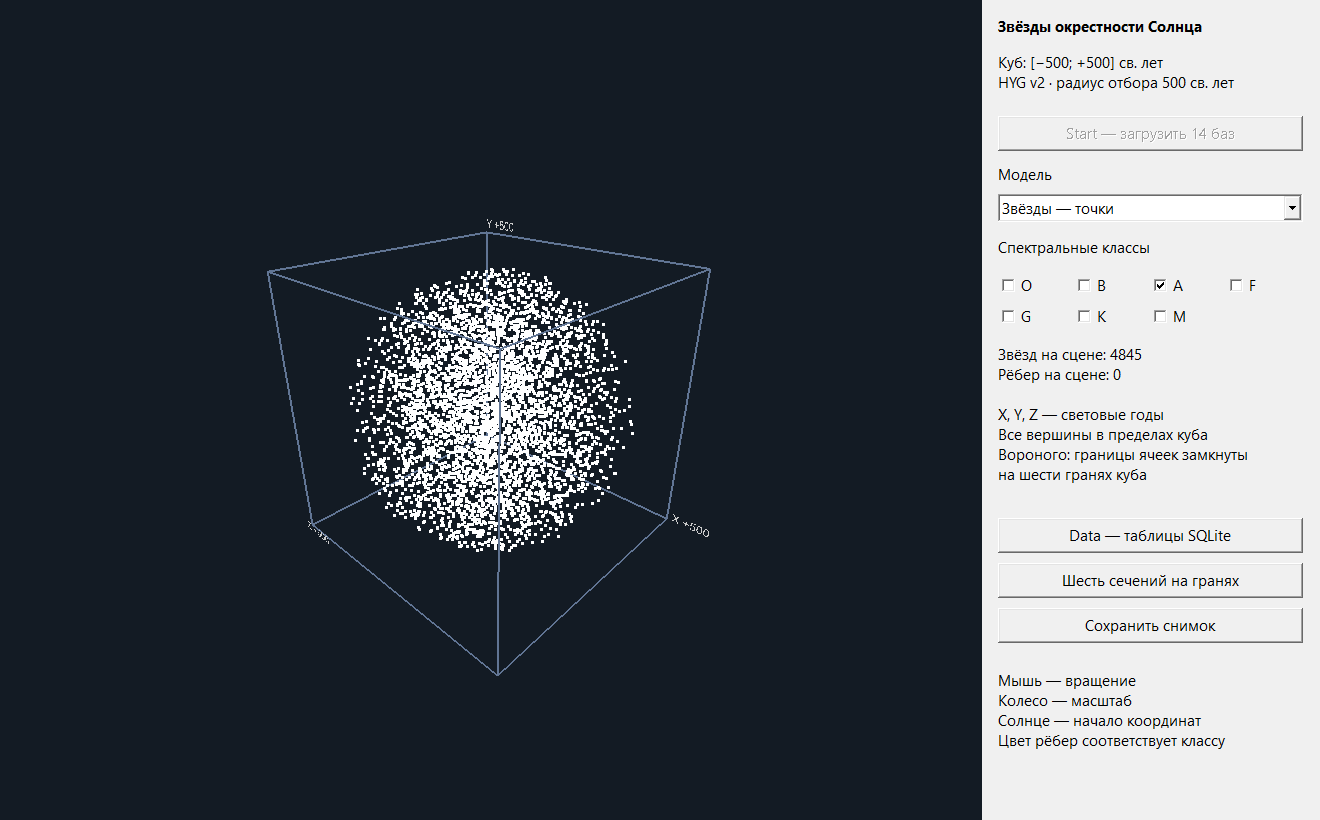
\includegraphics[width=\linewidth]{images/points-A.png}
\caption{Запуск приложения: точечная модель класса A, 4845 звёзд.}
\vspace{8pt}
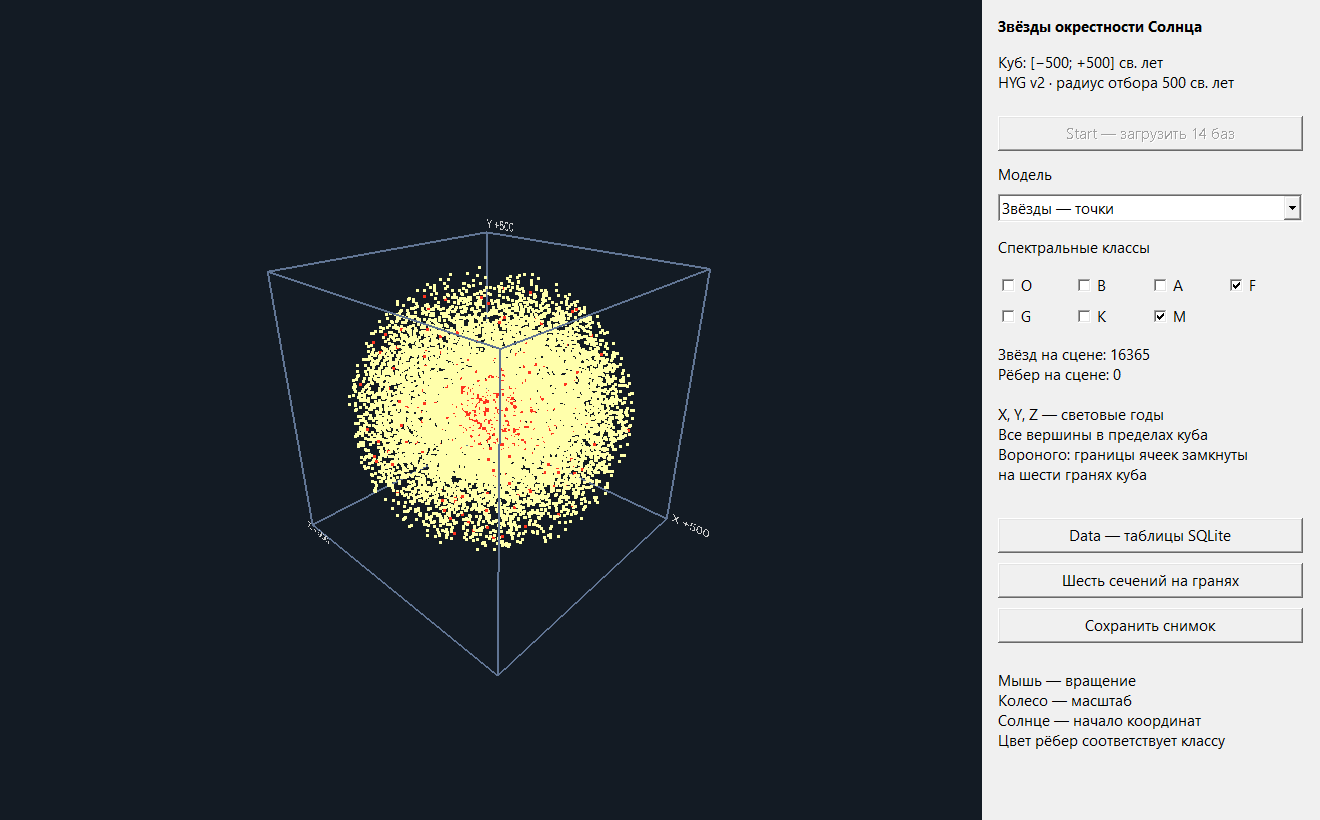
\includegraphics[width=\linewidth]{images/points-FM.png}
\caption{Совместный вывод точечных моделей F и M: 16\,365 узлов двух моделей.}
\end{figure}

\begin{figure}[p]
\centering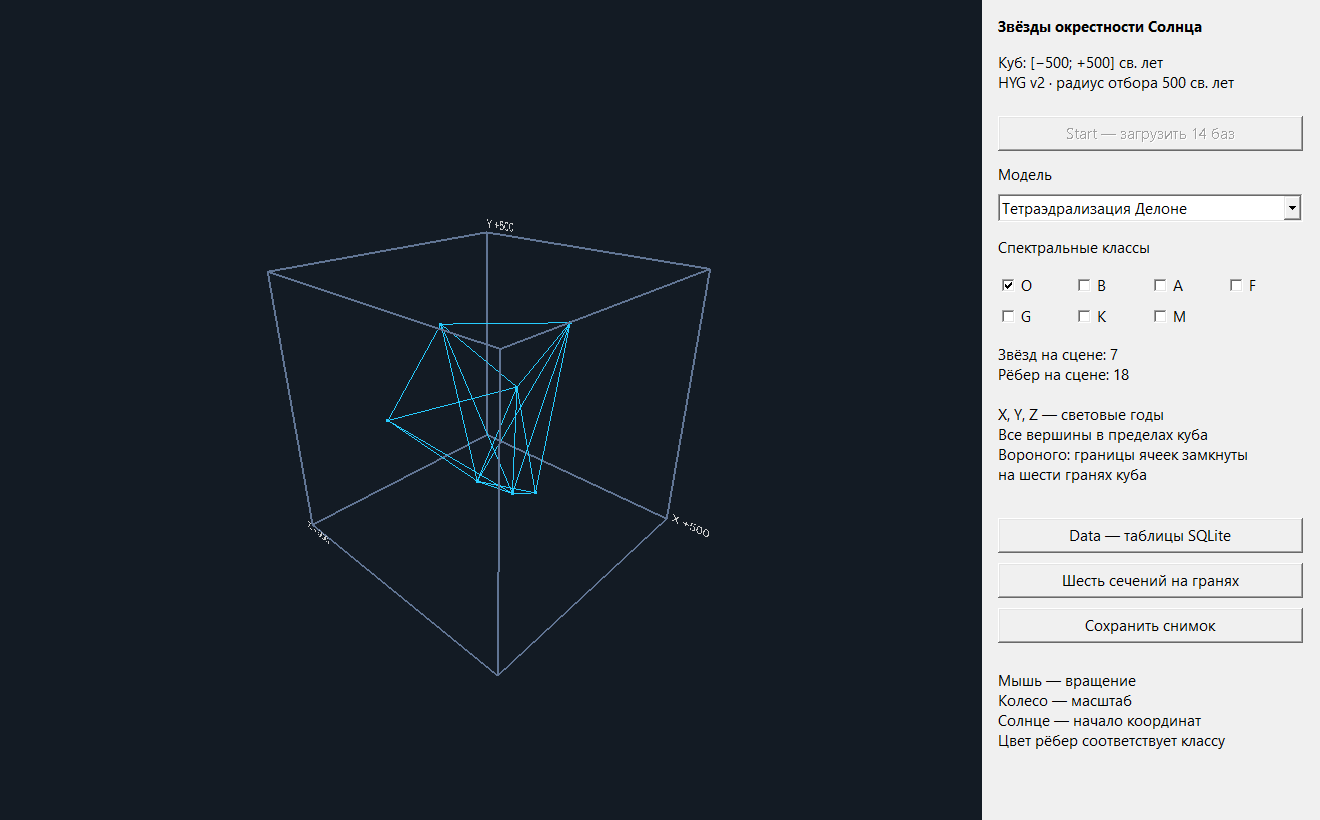
\includegraphics[width=\linewidth]{images/delaunay-O.png}
\caption{Тетраэдрализация класса O: 7 звёзд и 18 рёбер Делоне.}
\vspace{8pt}
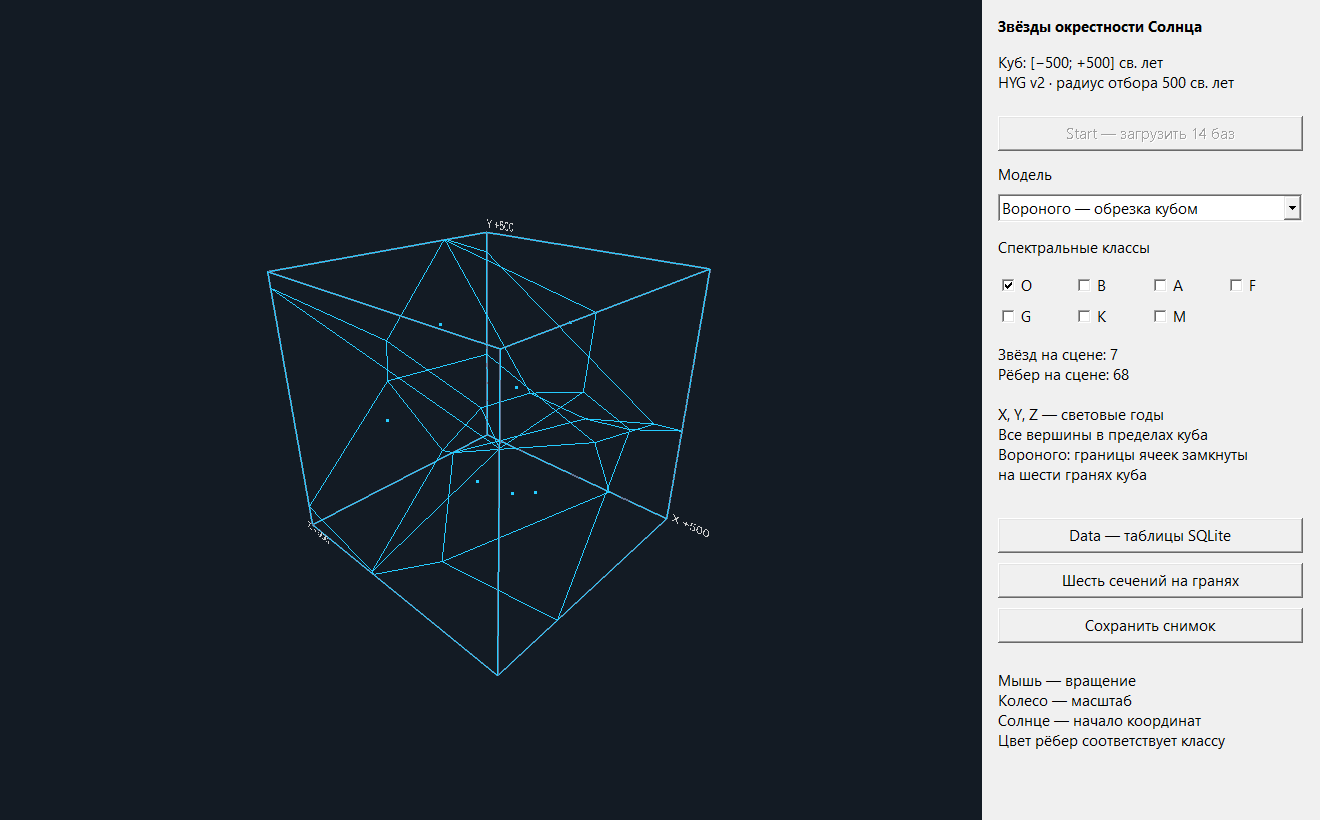
\includegraphics[width=\linewidth]{images/voronoi-O.png}
\caption{Ограниченная модель Вороного класса O: 68 рёбер, включая новые рёбра замыкания ячеек на кубе.}
\end{figure}

\begin{figure}[p]
\centering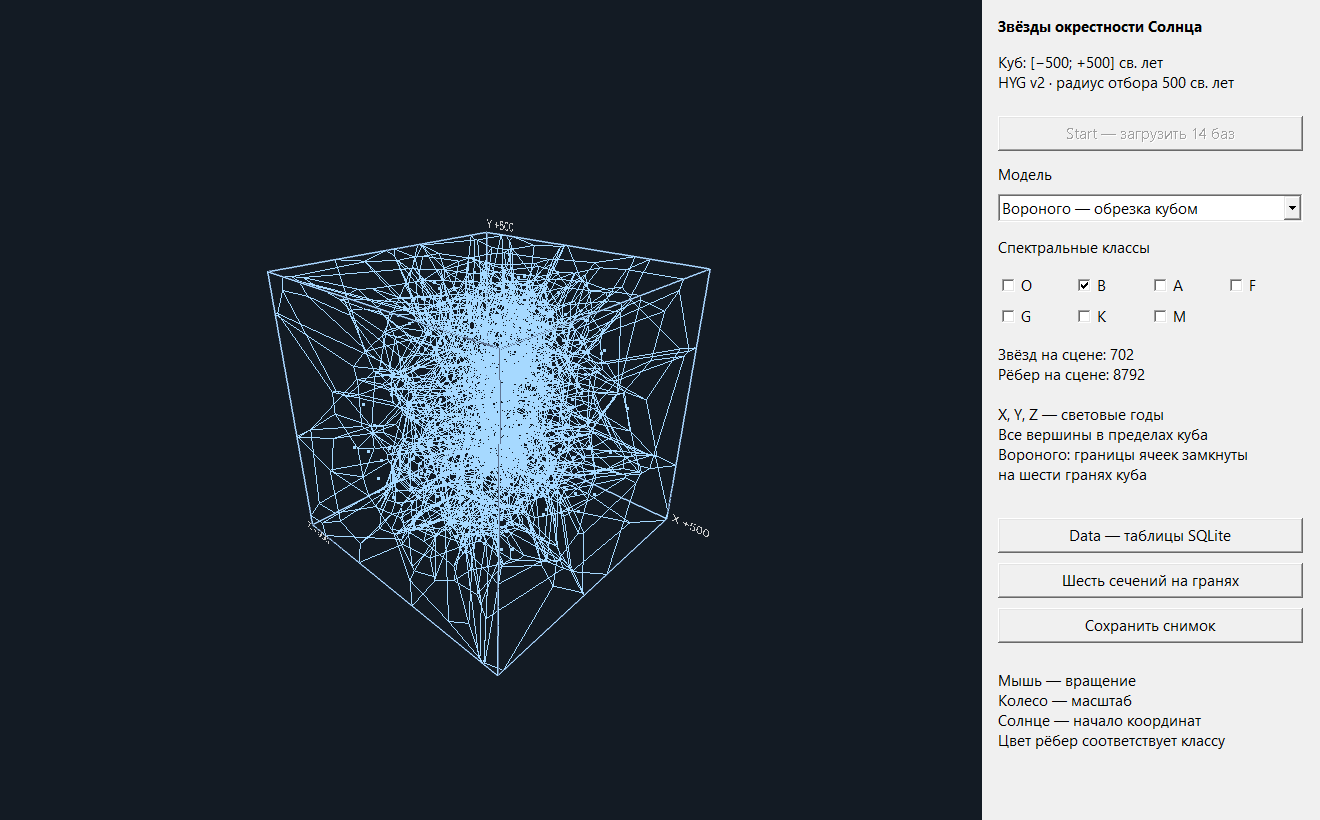
\includegraphics[width=\linewidth]{images/voronoi-B.png}
\caption{Модель Вороного класса B: 702 звезды и 8792 рёбра после ограничения и замыкания.}
\vspace{8pt}
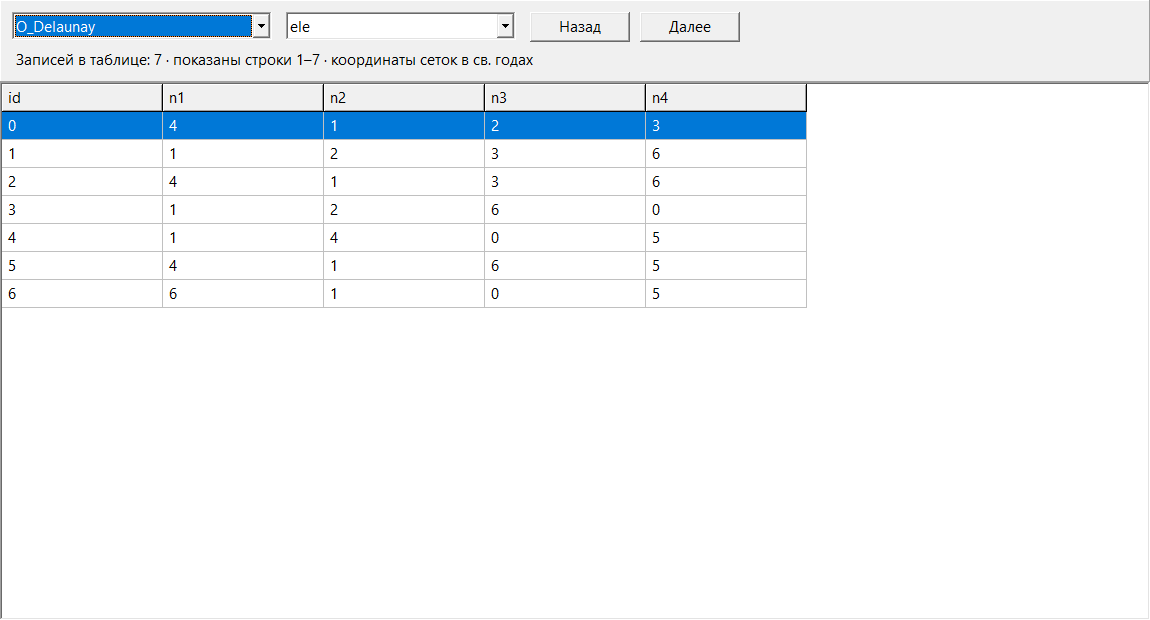
\includegraphics[width=\linewidth]{images/data-O.png}
\caption{Форма Data: просмотр таблицы тетраэдров класса O в SQLite.}
\end{figure}

\clearpage
\section{Проверка результата}
Для всех 267\,968 тетраэдров независимо вычислены центры описанных сфер. Поиск ближайшего узла по KD-дереву подтвердил отсутствие звёзд внутри этих сфер с относительным допуском $10^{-7}$. Сумма объёмов тетраэдров каждого класса согласована с объёмом выпуклой оболочки его узлов с относительным допуском $10^{-9}$.

Проверены координаты всех отображаемых рёбер Вороного: они принадлежат $[-500;500]$ с численным допуском $10^{-8}$ св. года. Для вершин и центроидов всех граничных многоугольников проверено, что соответствующая звезда является ближайшей среди всех узлов класса, с абсолютным допуском $10^{-6}$ св. года. Для класса O ячейки дополнительно пересчитаны с ограничениями от всех остальных звёзд, без использования соседства Делоне.

\begin{table}[ht]
\centering\small
\caption{Контроль объёма и покрытия границ для каждого класса}
\begin{tabular}{c|r|r|r}
Класс & Ячеек & $\sum_i\operatorname{Vol}V_i^C$, св. лет$^3$ & $\max|S_f-10^6|$, св. лет$^2$\\\hline
O & 7 & 1\,000\,000\,000 & $1.16\cdot10^{-10}$ \\
B & 702 & 1\,000\,000\,000 & $2.33\cdot10^{-10}$ \\
A & 4845 & 1\,000\,000\,000 & $3.49\cdot10^{-10}$ \\
F & 14291 & 1\,000\,000\,000 & $3.49\cdot10^{-10}$ \\
G & 11941 & 1\,000\,000\,000 & $2.33\cdot10^{-10}$ \\
K & 6718 & 1\,000\,000\,000 & $3.49\cdot10^{-10}$ \\
M & 2074 & 1\,000\,000\,000 & $1.16\cdot10^{-10}$

\end{tabular}
\end{table}

Для каждого класса сумма объёмов ячеек равна $10^9$ св. лет$^3$ с максимальной абсолютной погрешностью $1{,}20\cdot10^{-7}$. Сумма площадей многоугольников на каждой грани равна $10^6$ св. лет$^2$ с погрешностью не более $3{,}50\cdot10^{-10}$. Совместно с проверкой ближайшей звезды это подтверждает покрытие куба. Для всех 2494 исходных лучей и сохранившихся частей рёбер Вороного проверены три равноудалённые ближайшие звезды с относительным допуском $10^{-8}$. Проверка \code{PRAGMA integrity\_check} для всех 14 баз дала результат \code{ok}.

\section{Вывод}
В ходе лабораторной работы было выполнено построение сеточных моделей звёзд окрестности Солнца по каталогу HYG: рассчитаны тетраэдрализации Делоне и диаграммы Вороного семи спектральных классов с помощью TetGen, сформированы базы SQLite и реализована визуализация средствами GLScene. Модели ограничены кубом с ребром 1000 световых лет. Ячейки Вороного замкнуты по его граням, получены все шесть сечений мозаики для каждого класса. Корректность ограничения подтверждена проверками ближайших звёзд, объёмов ячеек и площадей граничных многоугольников.
\end{document}

